\documentclass[margin=10pt]{standalone}
%\usepackage{cmbright}
%\renewcommand{\familydefault}{\sfdefault}
\usepackage[T1]{fontenc}
\usepackage{lmodern}
\usepackage{color}


\usepackage{tikz}
\usetikzlibrary{arrows}
\usetikzlibrary{arrows.meta}
\usetikzlibrary{backgrounds}
\usetikzlibrary{decorations.markings}
\usetikzlibrary{fit}
\usetikzlibrary{matrix}
\usetikzlibrary{positioning}
\usetikzlibrary{shadows}

\begin{document}
{
\normalsize
%\large

\newsavebox\mybox
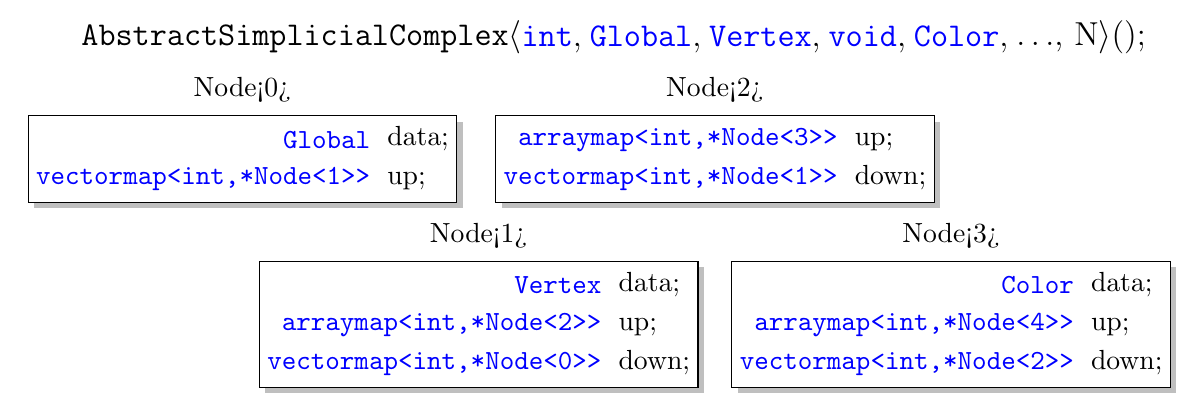
\begin{tikzpicture}[
		every node/.style = {
			draw,
			text height = 1.5ex,
			fill = white!5,
			align = center,
		},
		labeltxt/.style = {
			draw = none,
			fill = none,
			font=\fontsize{12}{12}\selectfont,
			inner sep = 0,
			outer sep = 0,
			%minimum height = 0.7cm,
		},
		simplex/.style = {
			drop shadow,
		},
		genmatrix/.style={
			matrix of nodes,
			nodes = {draw=none},
			nodes in empty cells,
			outer sep = 0.5mm,			% allow them to stack better
			inner sep = 0.5mm,
			minimum size = 0.5cm,
			column 1/.style={nodes={anchor=east}},
			column 2/.style={nodes={anchor=west}},
		},
		line/.style = {
			ultra thick,
		},
        ptr/.style = {
			postaction = {decorate,
				decoration={markings,
		            mark=at position 0.0
		                with {
		                    \filldraw[fill=black] circle[radius=0.5mm];
		                }
		        },
		    },
        },
        arr/.style = {
        	-Latex,
        },
 		]

	%\draw[step=1cm,black!80,very thin] (0,0) grid (16,12);
	%\draw[step=0.5cm,black!20,very thin] (0,0) grid (16,12);

	\node[labeltxt] (ASC) at (3cm,5cm) {\texttt{\textbf{AbstractSimplicialComplex$\langle$}}};
	\node[labeltxt, right=0mm of ASC] (arg1) {{\color{blue}\verb|int|},};
	\node[labeltxt, right=1mm of arg1.east] (arg2) {{\color{blue}\verb|Global|},};
	\node[labeltxt, right=1mm of arg2.east] (arg3) {{\color{blue}\verb|Vertex|},};
	\node[labeltxt, right=1mm of arg3.east] (arg4) {{\color{blue}\verb|void|},};
	\node[labeltxt, right=1mm of arg4.east] (arg5) {{\color{blue}\verb|Color|},};
	\node[labeltxt, right=1mm of arg5.east] (endASC) {$\ldots$, N$\rangle$();};

	\pgfmathsetlengthmacro{\bh}{2.25cm}
	\pgfmathsetlengthmacro{\ho}{3cm}
	\pgfmathsetlengthmacro{\bv}{3.5cm}
	\pgfmathsetlengthmacro{\hs}{0.4}

	%%%%%%%%%%%%%%%%%
	% Node<0>       %
	%%%%%%%%%%%%%%%%%
	\matrix[simplex,
			genmatrix,
			label={north:{Node<0>}}
			]
		(root) at (\bh,\bv)
	{
		{\ttfamily \color{blue} Global} & data;\\
		{\color{blue} \verb|vectormap<int,*Node<1>>|} & up;\\
	};

	%%%%%%%%%%%%%%%%%
	% Node<1>       %
	%%%%%%%%%%%%%%%%%
	\matrix[simplex,
			genmatrix,
			label={north:{Node<1>}}
			]
		(1) at (\bh+\ho,\hs*\bv)
	{
		{\ttfamily \color{blue} Vertex} & data;\\
		{\color{blue} \verb|arraymap<int,*Node<2>>|} & up;\\
		{\color{blue} \verb|vectormap<int,*Node<0>>|} & down;\\
	};

	%%%%%%%%%%%%%%%%%
	% Node<2>       %
	%%%%%%%%%%%%%%%%%
	\matrix[simplex,
			genmatrix,
			label={north:{Node<2>}}
			]
		(2) at (\bh+2*\ho,\bv)
	{
		{\color{blue} \verb|arraymap<int,*Node<3>>|} & up;\\
		{\color{blue} \verb|vectormap<int,*Node<1>>|} & down;\\
	};

	%%%%%%%%%%%%%%%%%
	% Node<3>       %
	%%%%%%%%%%%%%%%%%
	\matrix[simplex,
			genmatrix,
			label={north:{Node<3>}}
			]
		(3) at (\bh+3*\ho,\hs*\bv)
	{
		{\ttfamily \color{blue} Color} & data;\\
		{\color{blue} \verb|arraymap<int,*Node<4>>|} & up;\\
		{\color{blue} \verb|vectormap<int,*Node<2>>|} & down;\\
	};

\end{tikzpicture}
}% end size
\end{document}